\documentclass[prd,showpacs,twocolumn]{revtex4-1}
\usepackage{graphicx}% Include figure files
\usepackage{epstopdf}
\usepackage{dcolumn}% Align table columns on decimal point
\usepackage{bm}% bold math
\usepackage{amsmath}
%\nofiles
\begin{document}
\title{Relativistically induced divergence of electric field}
\author{Peifeng Wang}
\address{Mijiaqiao 34-1-5, Xi'an, Shaanxi, P. R. China 710075}
\address{Guanghua Road 1\#, 34-1-5 3rd floor, Yanta District, Xi'an, Shaanxi, P. R. China 710075}
\begin{abstract}
It is demonstrated that, divergence of electric field can vary due to relativistic transformation. Two approaches are presented with consistent outcomes. And it indicates that divergence of electric field may not be exclusively associated with electric charges, thus violates the Gauss law of Maxwell equations.
\end{abstract}
\pacs{03.50.De}
\maketitle
%249489

In general, vector fields have divergence and curl. In electrodynamics, the divergence of field has been known to be associated only with electric charges, as manifested by the Gauss law of the Maxwell equations.
\begin{eqnarray}
&&\nabla\cdot\mathbf{E}=\frac{\rho}{\epsilon_0}\nonumber\\
&&\nabla\cdot\mathbf{B}=0
\label{eqn:GaussLaw}
\end{eqnarray}
In an attempt to symmetrize electricity and magnetism, the divergence of magnetic field, i.e. magnetic charges\cite{Dirac,Schwinger}, has been extensively studied in both theories\cite{Hooft, Polyakov,Ginzburg,Rujula} and experiments\cite{Cabrera,Caplin,Pinfold,L3,D0,Fang} because it explains the quantization of electric charges. Whereas the divergence of electric field draws relatively little interest.

Although it has been observed that electric charge is invariant\cite{King}, we reveal a model in which divergence of electric field may be observed varying due to relativistic effect. One of our scheme is based on the observation that Lorentz transformation may cause electric and magnetic field interchange, at the same time, field components with looped field lines may induce radial field components when viewed from certain moving frame. Analysis of these observed radial fields shows that, divergence of electric field can vary in different observing frames. Alternatively, it is shown that spatially uniform current in one frame may appear uneven in a different frame, which is observed as varying charge density/divergence of electric field. Calculation shows that both approaches agree with each other in showing varying divergence.

In Gaussian unit, the transformation of electromagnetic fields from reference frame $F$ to frame $F'$ moving with velocity $\mathbf{v}$ relative to $F$ are\cite{Jackson}
\begin{eqnarray}
&&[\mathbf{E'}]_{\mathbf{x'},t'}=[\gamma(\mathbf{E}+\boldsymbol\beta\times\mathbf{B})-\frac{\gamma^2}{\gamma+1}\boldsymbol\beta(\boldsymbol\beta\cdot\mathbf{E})]_{\mathbf{x},t}\nonumber\\
&&[\mathbf{B'}]_{\mathbf{x'},t'}=[\gamma(\mathbf{B}-\boldsymbol\beta\times\mathbf{E})-\frac{\gamma^2}{\gamma+1}\boldsymbol\beta(\boldsymbol\beta\cdot\mathbf{B})]_{\mathbf{x},t}\nonumber\\
&&\boldsymbol\beta=\frac{\mathbf{v}}{c},\beta=|\boldsymbol\beta|,\gamma=\frac{1}{\sqrt{1-\beta^2}}
\label{eqn:FieldsTransformation}
\end{eqnarray}
which, in SI unit, becomes
\begin{eqnarray}
&&[\mathbf{E'}]_{\mathbf{x'},t'}=[\gamma(\mathbf{E}+c\boldsymbol\beta\times\mathbf{B})-\frac{\gamma^2}{\gamma+1}\boldsymbol\beta(\boldsymbol\beta\cdot\mathbf{E})]_{\mathbf{x},t}\nonumber\\
&&[\mathbf{B'}]_{\mathbf{x'},t'}=[\gamma(\mathbf{B}-\frac{\boldsymbol\beta}{c}\times\mathbf{E})-\frac{\gamma^2}{\gamma+1}\boldsymbol\beta(\boldsymbol\beta\cdot\mathbf{B})]_{\mathbf{x},t}
\label{eqn:SIFieldsTransformation}
\end{eqnarray}

The subscripts indicate that the left hand side are fields at $(\mathbf{x'},t')$ in frame $F'$, while the right hand side contains fields at $(\mathbf{x},t)$ in frame $F$. $(\mathbf{x'},t')$ and $(\mathbf{x},t)$ are related by Lorentz transformation
\begin{eqnarray}
&&ct'=\gamma(ct-\boldsymbol\beta\cdot\mathbf{x})\nonumber\\
&&\mathbf{x'}=\mathbf{x}+\frac{\gamma-1}{\boldsymbol\beta^2}\boldsymbol\beta(\boldsymbol\beta\cdot\mathbf{x})-ct\gamma\boldsymbol\beta
\label{eqn:LorentzTranformation}
\end{eqnarray}

Geometrically, the force lines of field with nonvanishing curl are closed loops, while fields with nonvanishing divergence has radial force lines. In eqn. (\ref{eqn:FieldsTransformation}), the terms $\gamma\boldsymbol\beta\times\mathbf{B}$ and $-\gamma\boldsymbol\beta\times\mathbf{E}$ show interchanges between electric field and magnetic field. They also represent transformations between azimuthal component and radial component of the fields, depicted in fig. \ref{fig:fieldtransformation}. As to be shown, the radial electric field $\mathbf{E}'$ in fig. \ref{fig:fieldtransformation}b has varying divergence in different observing frames.

\begin{figure}
\center
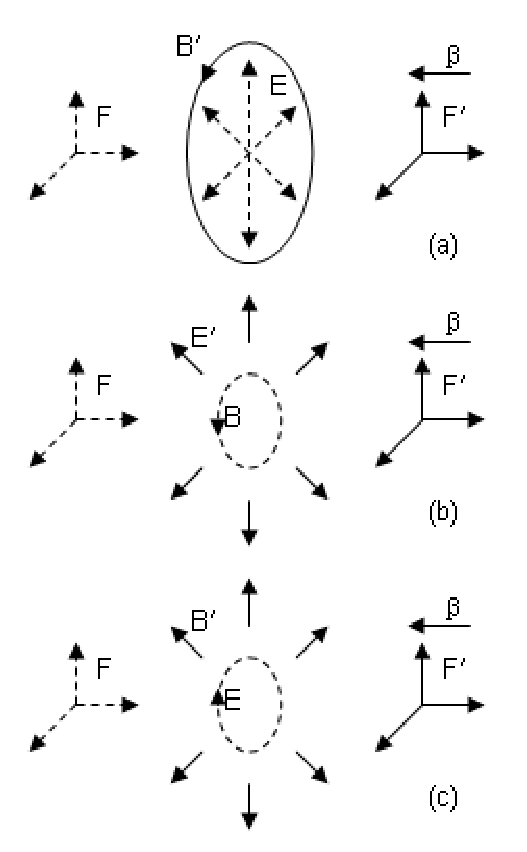
\includegraphics{f1.eps}
\caption{Dashed lines are fields observed in frame $F$, solid lines are fields observed in frame $F'$ moving with velocity $\boldsymbol\beta$ relative to frame $F$. (a) Radial component of field $\mathbf{E}$ induces circular shaped $\mathbf{B'}$. (b) $\boldsymbol\beta$ and $\mathbf{B}$ in frame $F$ form a left hand screw, circular shaped $\mathbf{B}$ induces outward pointing radial $\mathbf{E'}=\gamma\boldsymbol\beta\times\mathbf{B}$ in frame $F'$. (c) $\boldsymbol\beta$ and $\mathbf{E}$ in frame $F$ form a right hand screw, circular shaped $\mathbf{E}$ induces outward pointing radial $\mathbf{B'}=-\gamma\boldsymbol\beta\times\mathbf{E}$ in frame $F'$.}
\label{fig:fieldtransformation}
\end{figure}

\begin{figure}
\center
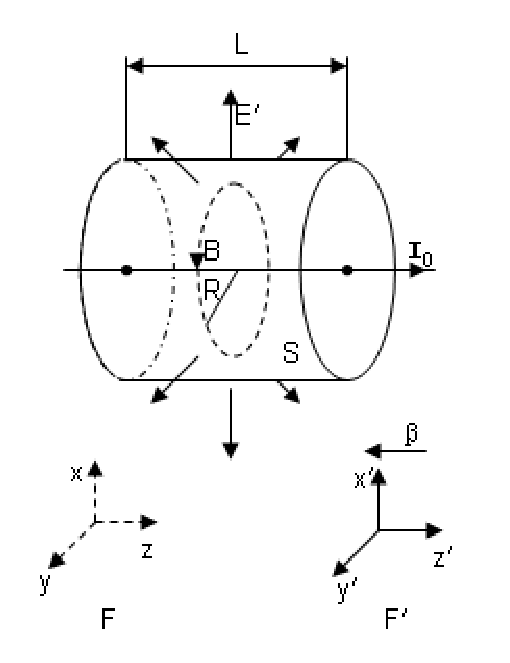
\includegraphics{DivE.eps}
\caption{Fields observed around a straight wire carrying static current $I_0$. Dashed line shows that in frame $F$, the force line of magnetic induction $\mathbf{B}$ is concentric circular. Solid lines are electric field $\mathbf{E'}$ observed in frame $F'$ moving with velocity $\boldsymbol\beta$ relative to frame $F$, and $\mathbf{E'}$ has only radial component.}
\label{fig:linecurrent}
\end{figure}

An infinite long current carrying straight wire is a physical setup of the model in fig. \ref{fig:fieldtransformation}b. Following we present two approaches of analyzing the field around a straight wire in different observing frames.

Around a long straight wire carrying a static current $I_0$, the force lines of magnetic induction $\mathbf{B}$ are concentric circular, as the dashed lines shown in fig. \ref{fig:linecurrent}. The magnitude of $\mathbf{B}$ is \cite{Jackson}
\begin{eqnarray}
&&|\mathbf{B}|=\frac{\mu_0}{2\pi R}I_0
\label{eqn:linecurrentB}
\end{eqnarray}
where $R$ is the perpendicular distance from the observation point to the wire. When viewed from a frame $F'$ moving along z axis, an electric field $\mathbf{E'}$ emerges, and by eqn. (\ref{eqn:SIFieldsTransformation}) its magnitude can be computed as
\begin{eqnarray}
&&|\mathbf{E'}|=c\gamma\beta\frac{\mu_0}{2\pi R}I_0
\label{eqn:linecurrentE}
\end{eqnarray}
Since $\mathbf{B}$ is loop shaped, $\mathbf{E'}$ is radial. This radial electric field induced by concentric circular shaped magnetic induction forms a realization of the field transformation shown in fig. \ref{fig:fieldtransformation}b.

Here is a computation of the flux of field $\mathbf{E'}$ through a closed cylindrical surface $S$ around the straight wire, as shown in fig. \ref{fig:linecurrent}, the cylidrical surface has length of $L$. We then notice that $\mathbf{E'}$ has only radial component, so the integral is calculated only on the side surface, then
\begin{eqnarray}
&&\oint_S\mathbf{E'}\cdot\mathbf{n}da=2\pi RL|\mathbf{E'}|=c\gamma\beta\mu_0 LI_0
\label{eqn:EPFlux}
\end{eqnarray}
in eqn. (\ref{eqn:EPFlux}) the field flux through closed surface varies with observing frame and can be nonvanishing even without net charge.

The divergence of the electric field $\mathbf{E'}$ in Frame $F'$ is
\begin{eqnarray}
&&\nabla'\cdot[\mathbf{E'}]_{\mathbf{x'},t'}\nonumber\\
&&=\nabla'\cdot[(\gamma(\mathbf{E}+c\boldsymbol\beta\times\mathbf{B})-\frac{\gamma^2}{\gamma+1}\boldsymbol\beta(\boldsymbol\beta\cdot\mathbf{E}))]_{\mathbf{x},t}
\label{eqn:EPDivergence0}
\end{eqnarray}

In frame $F$, $\mathbf{E}=0$ around the straight wire, then from eqn. (\ref{eqn:SIFieldsTransformation})
\begin{eqnarray}
&&[\mathbf{E'}]_{\mathbf{x'},t'}=[\gamma(c\boldsymbol\beta\times\mathbf{B})]_{\mathbf{x},t}
\label{eqn:EPFromB}
\end{eqnarray}

Since $\boldsymbol\beta$ is along the z axis, and z components of field $B_z=0,E'_z=0$, eqn. (\ref{eqn:EPDivergence0}) becomes
\begin{eqnarray}
&&\nabla'\cdot[\mathbf{E'}]_{\mathbf{x'},t'}=\nabla\cdot[\mathbf{E'}]_{\mathbf{x'},t'}=\nabla\cdot[\gamma(c\boldsymbol\beta\times\mathbf{B})]_{\mathbf{x},t}
\label{eqn:EDivergence2}
\end{eqnarray}
along with $\nabla\times\boldsymbol\beta=0$
\begin{eqnarray}
\nabla'\cdot[\mathbf{E'}]_{\mathbf{x'},t'}&&=-[c\gamma\boldsymbol\beta\cdot\nabla\times\mathbf{B}]_{\mathbf{x},t}\nonumber\\
&&=-[c\gamma\mu_0\boldsymbol\beta\cdot\mathbf{J}]_{\mathbf{x},t}
\label{eqn:EPDivergence}
\end{eqnarray}
thus the divergence of electric field observed in frame $F'$ depends on $\boldsymbol\beta$ and $\mathbf{J}$. When $\boldsymbol\beta$ is not perpendicular to $\mathbf{J}$, $\nabla'\cdot\mathbf{E'}$ is nonvanishing even if there is no net charge.

For the setup in fig. \ref{fig:linecurrent}, magnetic induction $\mathbf{B}$ has only x and y components, and $\mathbf{J}=\hat{\mathbf{z}}I_0\delta(x)\delta(y)$, with $\hat{\mathbf{z}}$ being the unit z vector. Therefore 
\begin{eqnarray}
&&\nabla\times[\mathbf{B}]_{\mathbf{x},t}=\mu_0\mathbf{J}=\mu_0\hat{\mathbf{z}}I_0\delta(x)\delta(y)
\label{eqn:BCurl}
\end{eqnarray}
then
\begin{eqnarray}
&&\nabla'\cdot[\mathbf{E'}]_{\mathbf{x'},t'}=-c\gamma\beta\mu_0 I_0\delta(x)\delta(y)
\label{eqn:EPDivergence3}
\end{eqnarray}

Though $\mathbf{E}=0$ thus $\nabla\cdot\mathbf{E}=0$ in frame $F$, for $\beta\ne 0$ the divergence of $\mathbf{E'}$ observed in frame $F'$ is none zero at z axis, which is equivalent to a line charge at z axis. In addition, as $\beta$ varies in different observing frame, the observed $\nabla'\cdot\mathbf{E'}$ varies.

The varying divergence in eqn. (\ref{eqn:EPDivergence}) originates from relativistic transformation. To illustrate further, we consider an alternative approach with a slightly different model, in which the current in frame $F$ is
\begin{equation}
I=I_0u(t)=
\begin{cases}
I_0,&t>0\\
0,&t<0
\end{cases}
\label{eqn:ISwitchOn}
\end{equation}
i.e. instead of a permenant current $I_0$, the current in the straight wire is uniformly switched on at $t=0$ in frame $F$, thus $\nabla\cdot\mathbf{J}=0$ at all moment.

\begin{figure}
\center
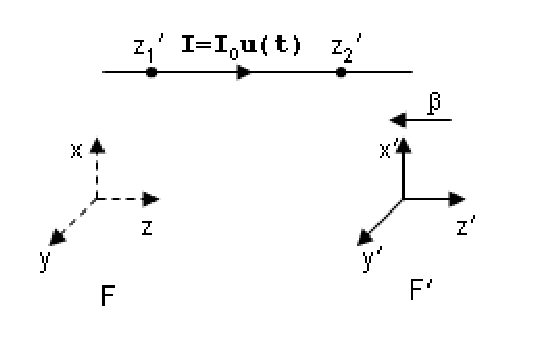
\includegraphics{SwitchOn.eps}
\caption{In frame $F$, the current is switched on uniformly over the whole wire at the same moment $t=0$. In frame $F'$, the event of switching on the current at $z_1'$ is observed at $t_1'$, and the event of switching on the current at $z_2'$ is observed at $t_2'$, $t_1'\ne t_2'$ when $z_1'\ne z_2'$. Therefore in Frame $F'$, the different switch-on time of the current leads to the observation of an accumulation of electric charge.}
\label{fig:SwitchOn}
\end{figure}

However, it is worth noting that in frame $F'$ the current at different $z'$ is switched on at different moments $t'$. In general, events happening at $(z, t)$ in frame $F$ are observed at $(z', t')$ in frame $F'$, where $(z, t)$ and $(z', t')$ are related by the Lorentz transformation (\ref{eqn:LorentzTranformation}). The current $I'$ observed in frame $F'$ is
\begin{eqnarray}
I'(z',t')=\gamma I_0u(\gamma(t'+\frac{\beta z'}{c}))
\label{eqn:IP}
\end{eqnarray}

In the current case, the event of switching on current at $z_1, t=0$ in frame $F$ is observed at $z'_1,t_1'$ in frame $F'$
\begin{eqnarray}
&&t_1'=-\gamma\frac{\beta z_1}{c}\nonumber\\
&&z_1'=\gamma z_1
\label{eqn:LorentzTranformation1}
\end{eqnarray}
and the event of switching on current at $z_2, t=0$ in frame $F$ is observed at $z'_2,t_2'$ in frame $F'$
\begin{eqnarray}
&&t_2'=-\gamma\frac{\beta z_2}{c}\nonumber\\
&&z_2'=\gamma z_2
\label{eqn:LorentzTranformation2}
\end{eqnarray}
without loss of generality, we assume $t_1'<t_2'$, then in frame $F'$, prior to $t_1'$, no current is observed at either $z_1'$ or $z_2'$, after $t_2'$, current of $\gamma I_0$ is observed at both $z_1'$ and $z_2'$. The most notable thing is that, during the period between $t_1'$ and $t_2'$, one observes current of $\gamma I_0$ only at $z_1'$ but no current at $z_2'$. As a result, electric charge accumulates between $z_1'$ and $z_2'$. The total accumulated charge is
\begin{eqnarray}
Q'=(t_2'-t_1')\gamma I_0=\frac{\gamma\beta}{c}(z_1'-z_2')I_0
\label{eqn:totalCharge}
\end{eqnarray}
That is, in frame $F'$, after $t_2'$ when the current is switched on at both $z_1'$ and $z_2'$, one observes net charge $Q'$ on the straight wire between $z_1'$ and $z_2'$. More interestingly, $Q'$ varies in different observing frame while $Q=0$ in frame $F$. To compute the charge density, we start with the current density $\mathbf{J'}$ in frame $F'$
\begin{eqnarray}
\mathbf{J'}(z',t')=\gamma\mathbf{\hat{z}} I_0u(\gamma(t'+\frac{\beta z'}{c}))\delta(x)\delta(y)
\label{eqn:JP}
\end{eqnarray}
the divergence of $\mathbf{J'}$ in frame $F'$ is
\begin{eqnarray}
\nabla'\cdot\mathbf{J'}=\gamma\frac{\gamma\beta}{c} I_0\delta(\gamma(t'+\frac{\beta z'}{c}))\delta(x)\delta(y)
\label{eqn:DivJP}
\end{eqnarray}
then with the continuity equation
\begin{eqnarray}
\frac{\partial\rho'}{\partial t'}=-\nabla'\cdot\mathbf{J'}=-\gamma\frac{\gamma\beta}{c} I_0\delta(\gamma(t'+\frac{\beta z'}{c}))\delta(x)\delta(y)
\label{eqn:rho_rate}
\end{eqnarray}
the charge density can be obtained by integral of eqn. (\ref{eqn:rho_rate})
\begin{eqnarray}
\rho'=-\frac{\gamma\beta}{c} I_0u(\gamma(t'+\frac{\beta z'}{c}))\delta(x)\delta(y)
\label{eqn:rho}
\end{eqnarray}
comparing with eqn. (\ref{eqn:JP}), the charge density in frame $F'$ is switched on at the same moment when the current is observed switched on. After the switch-on moment,
\begin{eqnarray}
\rho'=-\frac{\gamma\beta}{c} I_0\delta(x)\delta(y)
\label{eqn:static_rho}
\end{eqnarray}
Thus the charge density $\rho'$ also varies in different observing frames. In frame $F$ where $\beta=0$, the uniform switch-on of current at $t=0$ ensures that the charge distribution remains invariant zero. Whereas, in a different frame $F'$, the current is observed varying both spatially and temporally, which leads to divergence of current, thus varying charge density and divergence of electric field.

With $c^{-2}=\mu_0\epsilon_0$, the charge density in eqn. (\ref{eqn:static_rho}) appears exactly the source of the field in eqn. (\ref{eqn:EPDivergence}). Both equations show that the divergence of electric field varies in different frames. In eqn. (\ref{eqn:static_rho}), it seems that the observed divergence is due to the observed charge density. However, in deriving eqn. (\ref{eqn:EPDivergence}), only the Lorentz force plays a role, while the event of switching on current is only imaginary and unnecessary. Therefore the varying divergence in eqn. (\ref{eqn:EPDivergence}) may not be associated with any actual electric charge, thus violates eqn. (\ref{eqn:GaussLaw}).

%\begin{acknowledgments}
%I am grateful to my family for their support and encouragement.
%\end{acknowledgments}

\begin{thebibliography}{0}
\label{sec:TeXbooks}
\bibitem{Dirac} P. A. M. Dirac, Proc. R. Soc. London A 133, 60 (1931).
\bibitem{Schwinger} J. Schwinger, Phys. Rev. 144, 1087 (1966).
\bibitem{Hooft} G. 't Hooft, Nucl. Phys. B 79, 276 (1974).
\bibitem{Polyakov} A. M. Polyakov, JETP Lett. 20, 194 (1974).
\bibitem{Ginzburg} I. Ginzburg, A. Schiller, Phys. Rev. D 57, 6599 (1998).
\bibitem{Rujula} A. De Rujula, Nucl. Phys. B 435, 257 (1995).
\bibitem{Cabrera} B. Cabrera, Phys. Rev. Lett. 48, 1378 (1982).
\bibitem{Caplin} A. Caplin et al., Nature 321, 402 (1986).
\bibitem{Pinfold} J. Pinfold, R. Du, K. Kinoshita, B. Lorazo, B. Price, M. Regimbald, Phys. Lett. B 316, 407 (1993).
\bibitem{L3} L3 collaboration, M. Acciarri et al., Phys. Lett. B 345, 609 (1995).
\bibitem{D0} D0 collaboration, B. Abbott et al., Phys. Rev. Lett. 81, 524 (1998).
\bibitem{Fang} Z. Fang, N. Nagaosa, K. Takahashi, A. Asamitsu, R. Mathieu, T. Ogasawara, H. Yamada, M. Kawasaki, Y. Tokura, K. Terakura, Science 302, 92 (2003).
\bibitem{King} J. G. King, Phys. Rev. Lett. 5, 562 (1960).
\bibitem{Jackson} J. D. Jackson, Classical Electrodynamics, 3rd ed., (Wiley, New York, 1998).
\end{thebibliography}
\end{document}
